\chapter{Výsledky a porovnanie}

V tejto kapitole sa pozrieme na výkonnosť nášho riešenia v porovnaní
s CR-indexom. Testovanie prebehlo na tom istom počítači s procesorom
Intel Xeon CPU E5-2670 taktovaným na $2.60 GHz$.

Pre účely testovania sme používali dve sady vstupných dát. Prvou sadou sú
čítania získané nástrojom MiSeq z baktérie E.coli, kmeňa MG1655
získané od spoločnosti Illumina. Dĺžka genómu tejto baktérie je 4.7 miliónov bázových párov, čítania
majú viac akoako
stoosemdesiatnásobné pokrytie a chybovosť $0.75\%$. Druhú sadu tvoria čítania zo štrnásteho ľudského
chromozómu, získané z projektu GAGE \cite{gage}. Celková dĺžka reťazca je 107 miliónov bázových párov,
čítania majú štyridsaťdvanásobné pokrytie a chybovosť $1.5\%$.

Okrem týchto dvoch sád čítaní sme použili aj čítania náhodne generované z osekvenovaného
genómu baktérie E.coli s rôznou dĺžkou aj chybovosťou.

Testovali sme rýchlosť hľadania čítaní s daným podreťazcom a veľkosť štruktúr, ktoré potrebujeme pre odpovedanie
na takéto dotazy za rôznych podmienok. Pokiaľ nie je povedané inak, hodnota $k$ je $20$.

Podreťazce pre dotazy sme vygenerovali tak, aby $95\%$ podreťazcov
pochádzalo z náhodných čítaní a zvyšných $5\%$ boli úplne náhodné reťazce.

\begin{figure}

\centerline{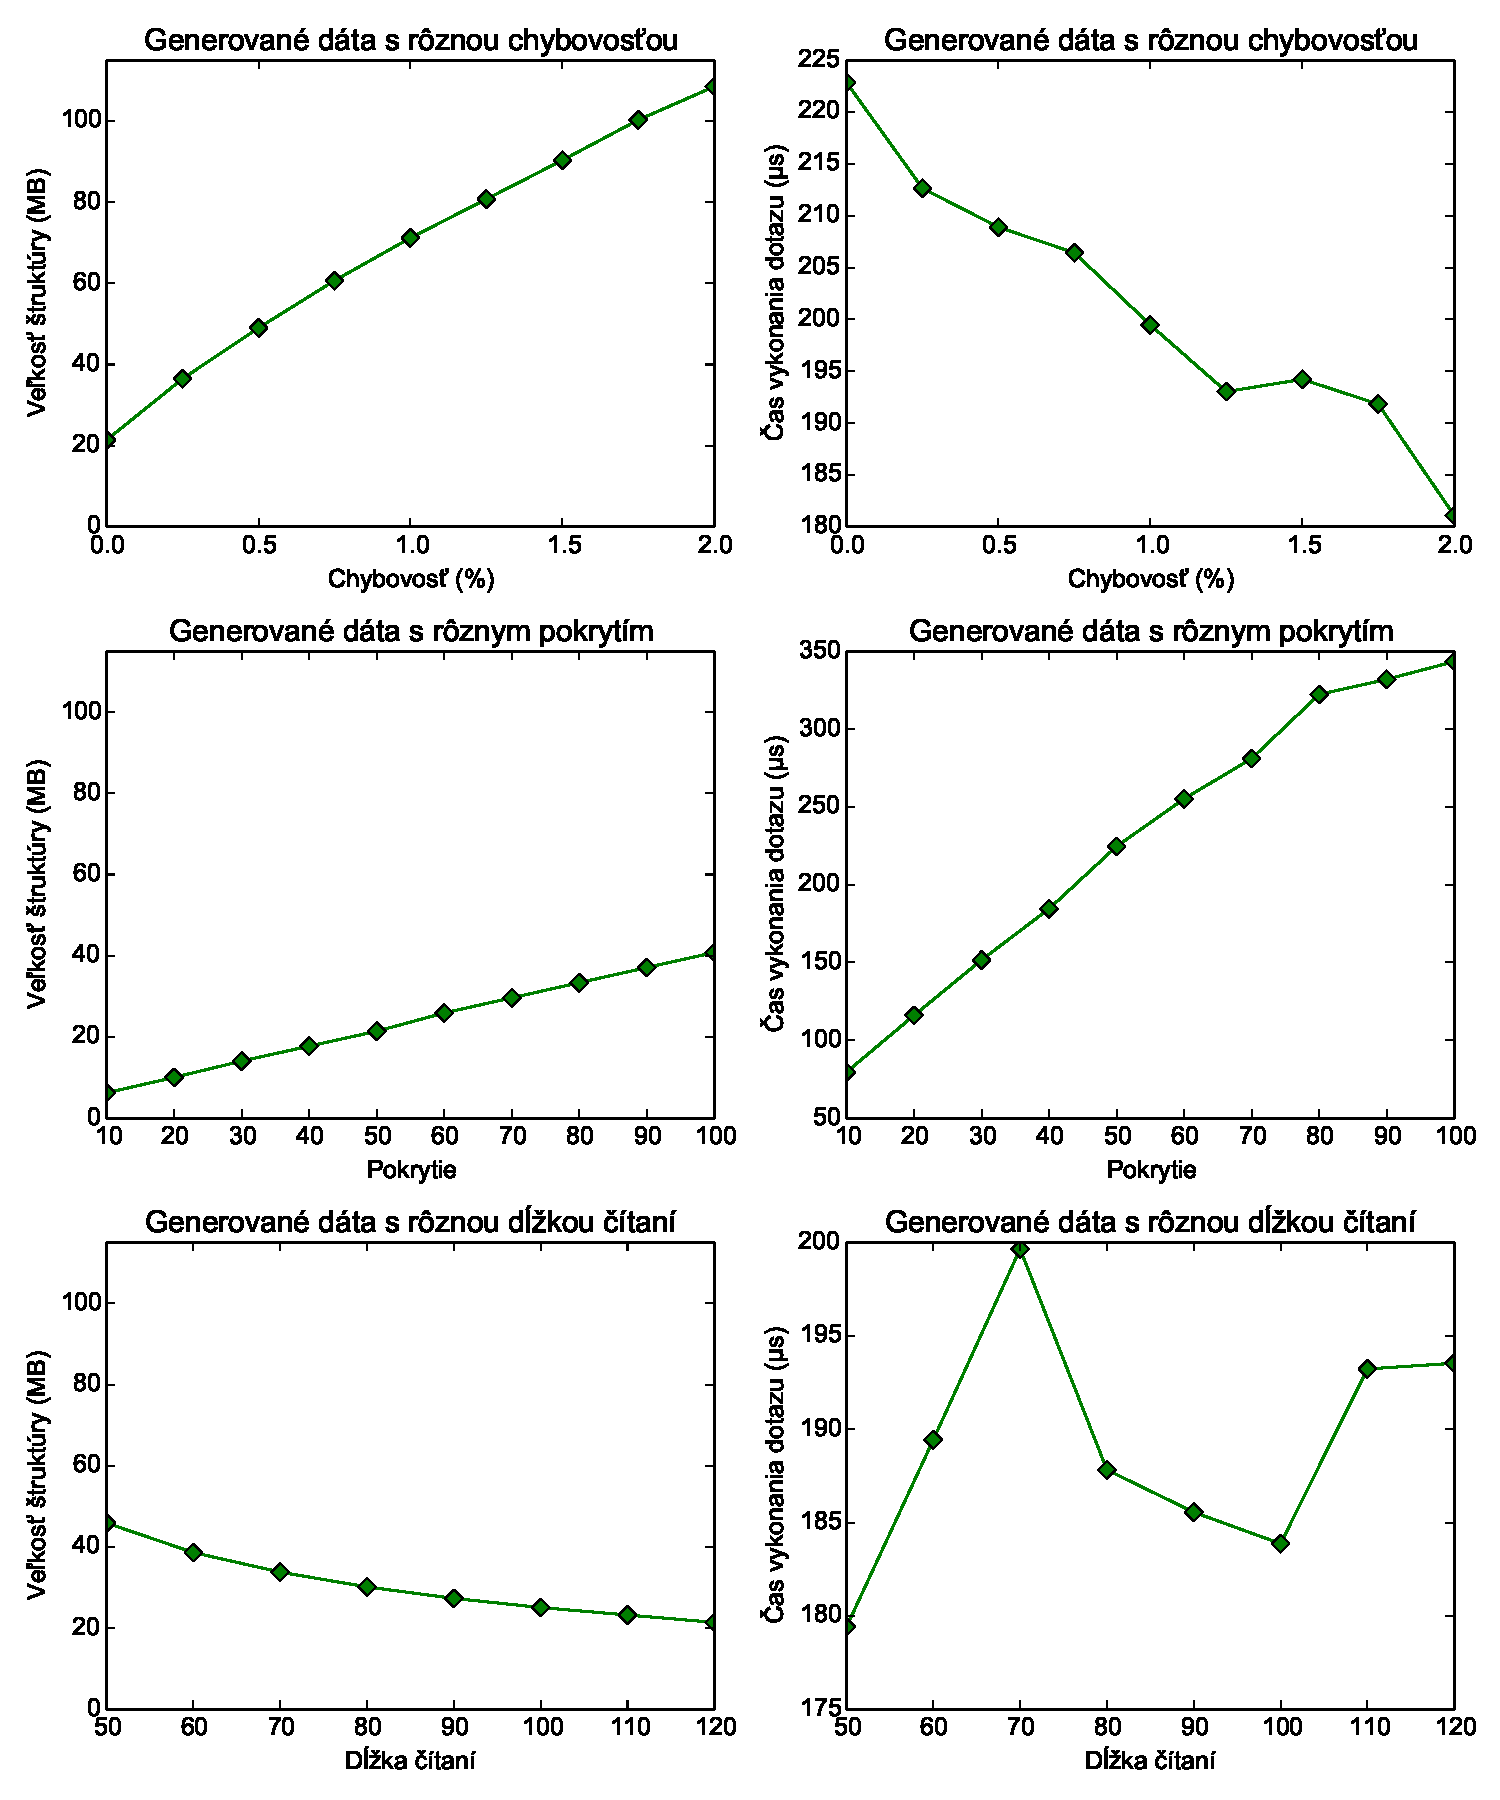
\includegraphics[width=1\textwidth]{images/chart_artificial.pdf}}

\caption[Simulované dáta]{Prvá dvojica tabuliek odzrkadľuje vplyv chybovosti dát na rýchlosť vykonávania dotazu a množstvo
pamäte potrebnej na uloženie všetkých pomocných štruktúr. Druhá dvojica ukazuje vplyv pokrytia,
tretia dvojica ukazuje vplyv dĺžky čítaní. Pri druhej a tretej dvojici tabuliek boli dáta generované
bez chýb.}

\label{chart:artificial}

\end{figure}

\section{Generované dáta}

Ako prvé si ukážeme naše simulované vstupné sady na obr. \ref{chart:artificial}. Ako prvé sme
generovali čítania dĺžky $120$ s rôznou šancou na chybné určenie bázy. Čítania mali
päťdesiatnásobné pokrytie. Ako druhé sme generovali čítania s rôznym pokrytím bez chýb.
Ako posledné sme generovali čítania s päťdesiatnásobným pokrytím líšiace sa v dĺžke
čítaní.

V prvej dvojici
tabuliek vidíme, že vyššia chybovosť spôsobuje zásadné zväčšenie celej štruktúry, ale
čas na vykonanie dotazu klesá. Za nárast pamäťovej náročnosti môžu dve skutočnosti. Prvou
je predĺženie $k$-nadslova, ktoré musí obsahovať všetky $k$-tice s chybou. Druhou je zväčšený
počet začiatkov, ktorý je spôsobený tým, že $k$-tice s chybou v čítaní sú oddelené od zvyšku
bez chyby. Za mierne zrýchlenie dotazov pri väčšej chybovosti je pravdepodobne zodpovedné
predĺženie $k$-nadslova, kvôli ktorému sa zníži priemerný počet začiatkov na pozíciu
v $k$-nadslove.

V druhej dvojici tabuliek vidíme, že vyššie pokrytie navyšuje aj pamäťové, aj časové nároky.
Pri každom pokrytí bola dĺžka $k$-nadslova takmer rovnaká, navyšoval sa iba počet začiatkov.
Z tohto dôvodu stúpal priemerný počet začiatkov na znak v $k$-nadslove, čím si vysvetľujeme
vyšší čas potrebný na vyriešenie dotazu.

V poslednej dvojici tabuliek vidíme, že dlhšie čítania sa našim postupom uložia na menej
miesta. Toto je spôsobené tým, že sa zmenší počet začiatkov. Zmeny v čase potrebnom na
riešenie dotazu sú malé a vysvetľujeme si ich ako náhodný šum.

\begin{figure}

\centerline{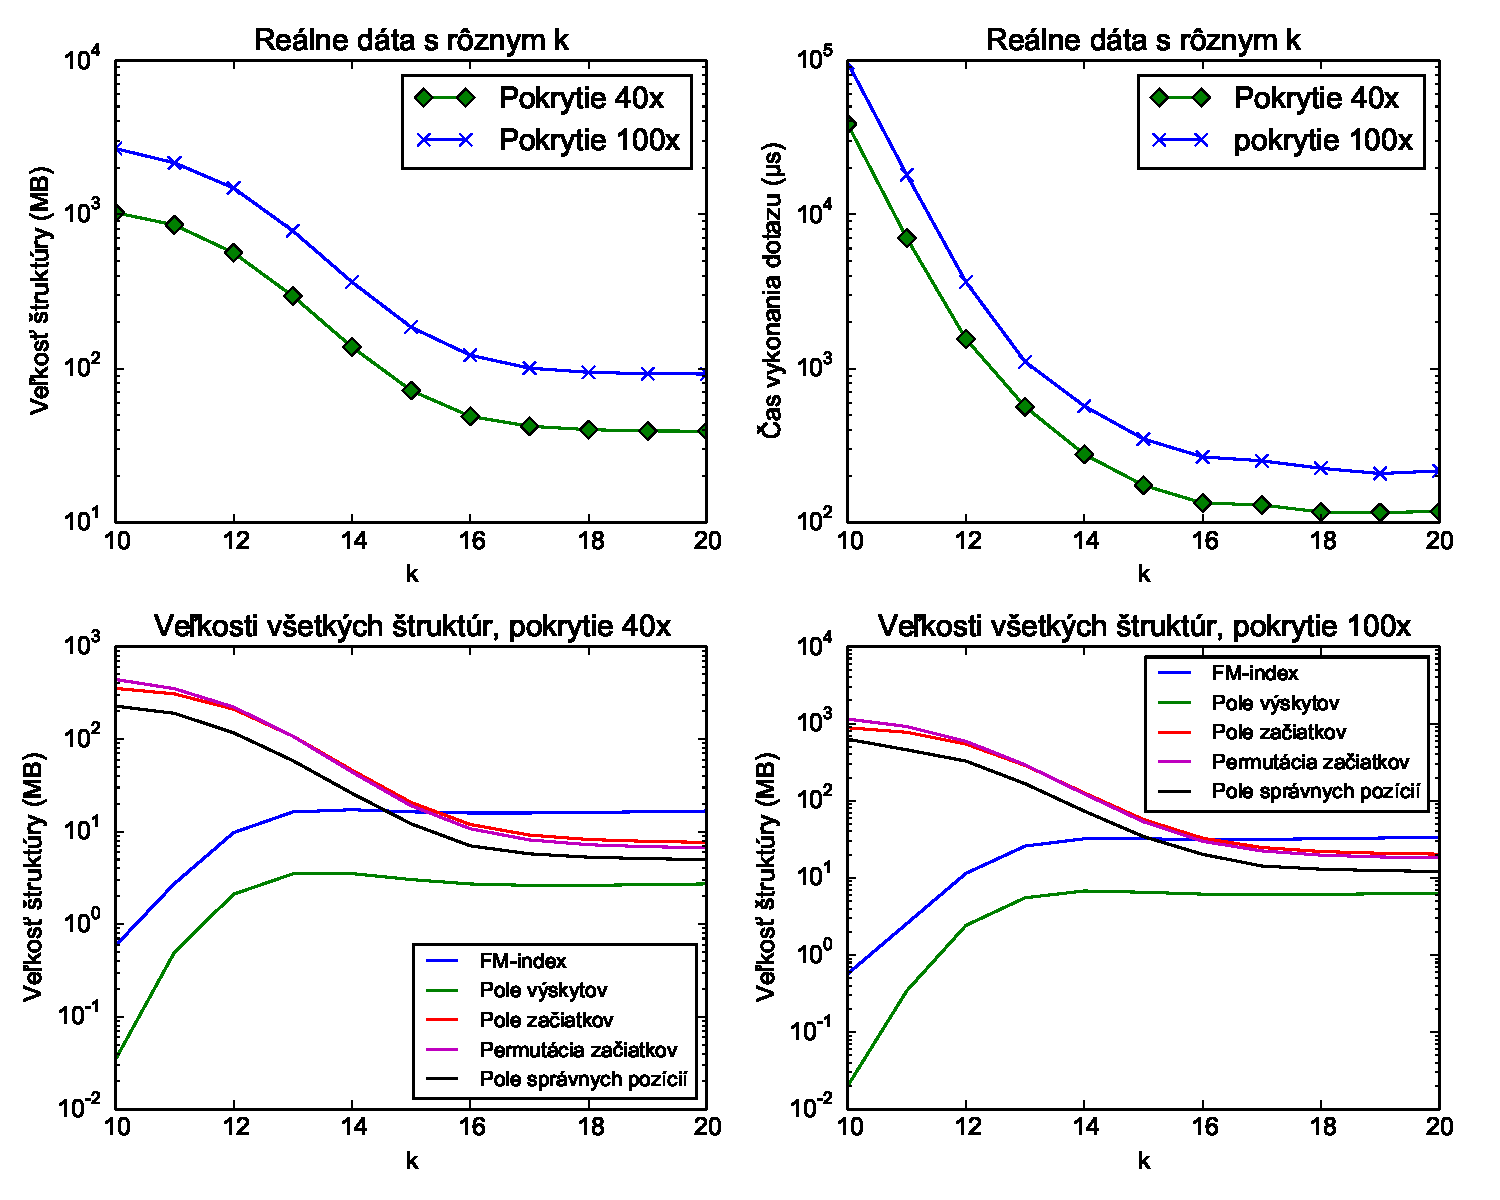
\includegraphics[width=1\textwidth]{images/chart_difks.pdf}}

\caption[E.coli dáta s rôznym $k$]{Výsledky testovania na čítaniach baktérie E.coli pre rôzne $k$.
V prvých dvoch tabuľkách je znázornený vplyv hodnoty $k$ na
pamäťové nároky štruktúry a čas spracovávania dotazu. V treťej tabuľke sú znázornené veľkosti
jednotlivých polí a štruktúr, ktoré používame, v závislosti od $k$ pri $40$-násobnom pokrytí,
v štvrtej pri $100$-násobnom pokrytí. Kvôli veľkému rozsahu nameraných hodnôt sú veľkosti
aj čas udávané v logaritmickej škále.}

\label{chart:difks}

\end{figure}

\section{Rôzne $k$}

Na druhej sade testov si ukážeme, aký vplyv má hodnota $k$ na veľkosť a rýchlosť celej štruktúry na obr. \ref{chart:difks}.
Tentokrát sme použili podmnožinu čítaní pre baktériu E.coli so štyridsať- a stonásobným pokrytím.

Pre malé hodnoty $k$ máme vysokú pravdepodobnosť, že sa rôzne časti genómu budú zhodovať v $k$-ticiach.
Dôsledok môžeme pozorovať v tabuľkách. Zatiaľčo dĺžka $k$-nadslova je rekordne malá, jednotlivé
čítania sú roztrúsené po tomto $k$-nadslove, čo má za efekt veľmi veľký počet začiatkov.

Pre rastúce
$k$ spočiatku rastie dĺžka nadslova, až sa pri $k \ge 15$ ustáli na takmer rovnakej hodnote. Zároveň
môžeme pozorovať, že pre $k \ge 16$ sa takmer vôbec nemení ani počet začiatkov. Tento fakt si
vysvetľujeme tak, že pre takéto $k$ začína $k$-nadslovo pomerne dobre reprezentovať celý genóm
E.coli. Rovnako ako s rastúcim $k$ klesá počet začiatkov, klesá aj čas spracovávania dotazu, čo len
potvrdzuje, že táto rýchlosť závisí od počtu skontrolovaných potenciálnych začiatkov.

\begin{figure}

\centerline{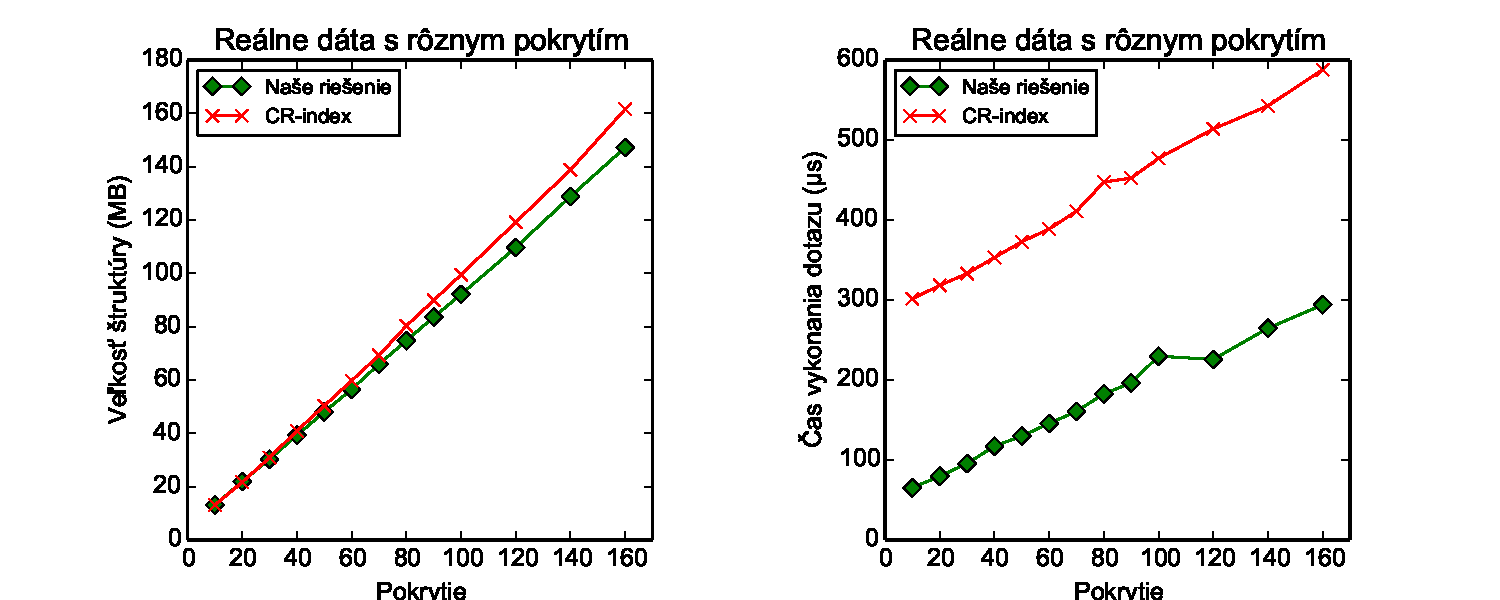
\includegraphics[width=1\textwidth]{images/chart_srcr.pdf}}

\caption[Porovnanie CR-indexu a našej štruktúry]{Porovnanie pamäťovej a časovej náročnosti
CR-indexu a nášho riešenia na čítaniach baktérie E.coli pri rôznom pokrytí.}

\label{chart:srcr}

\end{figure}

\section{Porovnanie s CR-indexom}

Ako posledné si ukážeme porovnanie nášho riešenia s CR-indexom na obr. \ref{chart:srcr}.
Z čítaní z baktérie E.coli sme náhodne povyberali podmnožiny s daným pokrytím. Pri každom
pokrytí používalo naše riešenie o trochu menej pamäte, napriek tomu bolo o viac než $200\mu s$
rýchlejšie. Tento výsledok však pripisujeme tomu, že sme zvolili vysoké $k$, keďže naša
štruktúra si vie lepšie poradiť s väčším $k$, zatiaľčo CR-index si vie lepšie poradiť s menším
$k$.

Podobne sme otestovali oba programy na čítaniach z ľudského chromozómu 14. CR-index na týchto čítaniach
potreboval $1.2GB$ pamäte, zatiaľčo naša štruktúra potrebovala až vyše $2.1GB$. Z časového hľadiska
to vyšlo naopak, CR-index potreboval okolo $21ms$ na spracovanie dotazu, zatiaľčo naša štruktúra
to zvládla v priemere za $9ms$.
